\documentclass[12pt]{article}
\usepackage[utf8]{inputenc}
\usepackage{hyperref}
\usepackage{graphics, graphicx}
\usepackage{fullpage}
\title{\textbf{Adiutor}}
\author{Mayank Mittal (190030026) \\ Mohammad Sameer (190010024)\\ E J V S Sathvik Goud (190010017)}
\date{08 December 2020}

\begin{document}

\maketitle

\section{Introduction}
Our project adiutor is a handy tool for students and teachers. Our project can be broken into the following points : 
\begin{description}
    \item[events] They are reminders for major events that take place in campus. Anyone(student or faculty) can request for events to be posted while only an Event Coordinator can accept or deny the event requests. Event Coordinator is a role which is given to an individual(faculty or student).
    \item [deadlines] They are reminders for the deadlines of assignments or other things posted by teachers for students to view and manage in their home pages.
    \item [room allotment] Faculty can view the existing room occupancy info  and request a room for a limited time. The requests for the room allotment are handled by the admin.
    \item [login] There are three modes of login - admin, student and faculty. Event coordinator page can be accessed after a student or faculty login.
\end{description}

\section{Programming Languages/Tools}
\subsection{Web Designing}
\begin{description}
    \item[HTML5] Basic design and other features like forms, tables etc.
    \item[Bootstrap CSS] For styling the webpages
\end{description}

\subsection{Server Side Scripting Language}
\begin{description}
    \item[PHP] The language used to interact with database
\end{description}

\subsection{Database}
\begin{description}
    \item[MySQL] For database management
\end{description}

\subsection{HTTP Server}
\begin{description}
    \item[Apache Server(XAMPP)] Server for running the PHP files
\end{description}

\subsection{Hosting Files and Version-control}
\begin{description}
    \item[GitHub] Hosting files, facilitate working with team members and version-control
\end{description}

\section{Compatibility of this Project}
This project is made and tested on \textbf{localhost}. So it is compatible on localhost network provided all the files of this  \href{https://github.com/samiitdh/SSL_Project}{repository} are present.

\section{Access to Adiutor}
Admin is in the database by default. The login credentials of admin are - Username: 69420 and Password: phpmyadmin. Once admin is logged in, he can add students or faculty through an html form. The username is their roll number and their default password is: \$role\_\$roll.no (where \$role is student or faculty and \$roll.no is the rollnumber of the individual) which can be changed later.

\section{Modes of Login}
The homepages for admin, faculty, students and event coordinator are all different. 
\begin{description}

    \item[admin] Admin can add individuals or courses to the database and can assign event coordinator role to an individual. Admin can also view the room occupancy and accept/deny room requests made by faculty.
    \item [student] Students can see major events posted in the events page and add them to their homepages with the click of a button. Students have their deadlines and events they added displayed in their homepage.Deadlines have a 'Mark as Done' button which clears the corresponding deadline from the homepage. They can request event coordinator to post an event.
    \item [faculty] The faculty can view and add deadlines to their courses. Faculty can view deadlines of other courses (taught by other faculty) too. They can view the room occupancy info and send request for a room for a time period. They have their desired events displayed in their homepage.
    \item [event coordinator] Event Coordinator is a role given to a student or a faculty member. Event Coordinator can view and manage event requests posted by other individuals. The homepage of event coordinator can be accessed from the homepage of a faculty or student.
\end{description}

\section{Implementation Files}
These are the list of files we used in this project:
\begin{description}
\item[init.php, dbcom.php] Create a connection with the database
\item[insert.php] Insert admin credential entries into the database
\item[login.php, logout.php] For login and logout
\item[validate.php] Checks if the entered login credentials are valid and if yes, redirects to corresponding homepages
\item[change\_pswd.php, change\_pswd\_helper.php ] Change the password of an account
\item[home\_admin.php] Homepage of the admin
\item[admin\_view.php] Page for admin to view existing accounts
\item[delete.php] Used by admin to delete an account
\item[add\_individual.php, add\_individual\_helper.php] Here admin can add an individual to the database
\item[add\_students.php, student\_varification.php] These files facilitate admin to add student for a course
\item[event\_coordinator.php, event\_coordinator\_helper.php] Admin can view the list of event coordinators, delete an existing event coordinator and add a new event coordinator
\item[admin\_room.php] Admin can view the room occupancy info here
\item[admin\_roomreq.php] Admin can manage room requests here
\item[add\_courses.php] Courses can be added to database by admin
\item[course\_validation.php] Checks the form data given to add\_courses.php
\item[view\_courses.php] Admin can view the courses in the database
\item[search.php] Admin can search for individuals here
\item[delete\_course.php] Admin can delete a course from the database
\item[home\_faculty.php] Homepage for faculty
\item[home\_student.php] Homepage for students
\item[view\_events.php] Individual can view posted events here and add them to be displayed in his/her homepage
\item[faculty\_room.php] Faculty can view the room allocation info here
\item[room\_req.php] Faculty can send a request for a room to the admin here
\item[faculty\_courses.php] Faculty can view and delete deadlines for the courses they teach
\item[new\_deadine.php] Faculty can add a new deadline for a course here
\item[deadline\_validation.php] This page checks the form data for a new deadline
\item[faculty\_deadlines.php] Here faculty can view deadlines of every course (including courses not taught by them)
\item[home\_eventco.php] Homepage of event coordinator
\item[add\_events.php] Event coordinator can add new events here
\item[event\_req.php] Event coordinator can view requests of events posted by others which can be accepted or denied
\item[eventco\_view.php] Event coordinator can view existing posted events which can be deleted
\end{description}

\section{Database}
A single database called "adiutor" was used for storing data. Different tables part of this data base are show below:

\begin{description}
    \item [individual] This table stores the basic information of all individuals
    \item [\$rollno\_events] This table stores the events that the individual with \$rollno as roll number added to his homepage
    \item [rooms] The table that stores room occupancy data
    \item [room\_reqs] This table is for storing room requests
    \item [\$rollno\_deadlines] This table stores the deadlines added by the faculty for his course where \$rollno as his roll number
    \item [events] The table for storing all the posted evens
    \item [event\_reqs] The table for storing the event requests made by individuals
    \item [courses] The table for storing the info about all available courses
    \item [\$rollno\_course] It stores the student info who take the course taught by the faculty whose roll number is \$rollno
\end{description}

\subsection{Columns for the above mentioned tables}
The columns of the tables are as shown in the below figures:
\begin{figure}[!ht]
\center
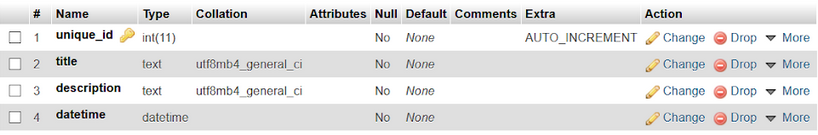
\includegraphics [width = 0.8\textwidth]{events}
\caption{Columns for events, \$rollno\_events and event\_reqs tables}
\label{fig:e}
\end{figure}

\begin{figure}[!ht]
\center
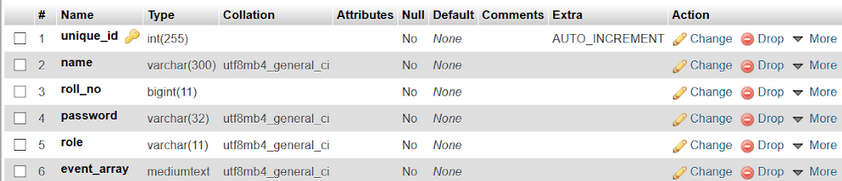
\includegraphics [width = 0.8\textwidth]{individual}
\caption{Columns for individual table}
\label{fig:i}
\end{figure}

\begin{figure}[!ht]
\center
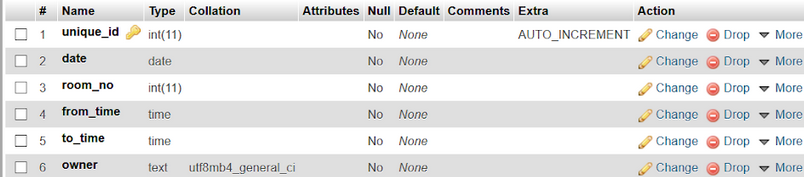
\includegraphics [width = 0.8\textwidth]{rooms}
\caption{Columns for rooms and room\_reqs tables}
\label{fig:r}
\end{figure}

\begin{figure}[!ht]
\center
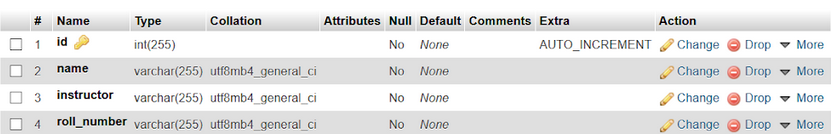
\includegraphics [width = 0.8\textwidth]{courses}
\caption{Columns for courses table}
\label{fig:c}
\end{figure}

\begin{figure}[!ht]
\center
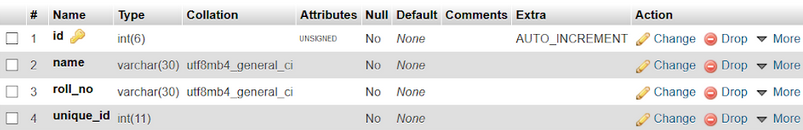
\includegraphics [width = 0.8\textwidth]{student}
\caption{Columns for \$rollno\_course table}
\label{fig:s}
\end{figure}

\begin{figure}[!ht]
\center
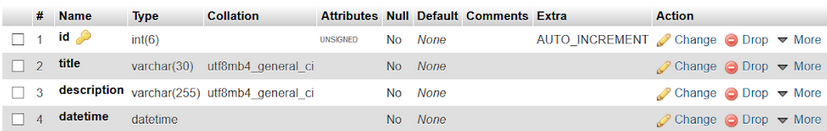
\includegraphics [width = 0.8\textwidth]{deadline}
\caption{Columns for \$rollno\_deadlines table}
\label{fig:d}
\end{figure}

\end{document}
